\documentclass[12pt,twoside]{article}

% packages
\usepackage{amssymb,amsmath,amsbsy}
\usepackage{graphicx}
\usepackage[includeheadfoot, top=1in, bottom=1in, hmargin=1in]{geometry}
\usepackage{fancyhdr}
\usepackage{verbatim}
\usepackage{url}
\usepackage{enumitem}
\usepackage{multicol}

% commands
\newcommand{\given}{\,|\,}
\newcommand{\dd}{\mathrm{d}}
\newcommand{\msun}{\mathrm{M}_\odot}
\newcommand{\projectname}[1]{\begin{center} {\huge {#1}} \end{center}}
\newcommand{\kms}{\mathrm{km}~\mathrm{s}^{-1}}

% environments
\newcommand{\problemname}{Problem}
\newcounter{problem}
\newenvironment{problem}{\paragraph{\problemname~\theproblem:}\refstepcounter{problem}}{}
 
\pagestyle{fancy}

\lhead{Due: Dec. 3 2014}
\chead{}
\rhead{}
\lfoot{Galactic Dynamics}
\cfoot{\thepage}
\rfoot{Fall 2014}

\begin{document}

\projectname{Project 3}

The goal of this problem set is to perturb stable disks and see what kind of resultant morphologies we get from secular perturbations (a bar) and external perturbations (a satellite galaxy). Before we can start analyzing such time-dependent processes, we have to modify our integration code from the previous assignment to handle passing around the present time. Feel free to do this on your own if you'd like, but I've included a Leapfrog integration function (in the attached Python module) along with an example acceleration function in case you were having issues with your integrator in the last assignment. 

\begin{problem} 

We'll start by implementing a time-dependent, bar-like potential in Python and look at how a disk of circular orbits reacts to this potential. For a background potential, we'll use the Isochrone potential:
\begin{equation}
	\Phi_{\rm iso}(r) = \frac{-G M}{b + \sqrt{b^2+r^2}}
\end{equation}
and set $GM=1$ and $b=1$ for simplicity. The bar potential we'll use comes from a set of bi-orthonormal potential-density pairs from Kalnajs (1976):
\begin{equation}
	\Phi_{\rm bar}(r,\phi) = \psi(r) \cos(2(\phi - \Omega_p t))
\end{equation}
where $\phi$ is just the azimuthal angle, $\Omega_p$ is the pattern speed of the bar, and

\begin{equation}
	\psi(r) = \epsilon \times
	\begin{cases}
	    -0.53\left(\frac{r}{a}\right)^2 \left[ 1 - 2.5\left(\frac{r}{a}\right)^2 + 2.1875\left(\frac{r}{a}\right)^4 - 0.65625\left(\frac{r}{a}\right)^6 \right] ,& r < a\\
	    0.017\left(\frac{r}{a}\right)^{-4},   &  r \geq a
	\end{cases}.
\end{equation}
Here, $\epsilon$ is the bar strength and $a$ is the scale length of the bar. The total potential is just
\begin{equation}
	\Phi = \Phi_{\rm iso} + \Phi_{\rm bar}.
\end{equation}

Write functions to compute the energy and acceleration from this potential. Make plots of isopotential contours along $z=0$ in the $x-y$ plane (e.g., using \texttt{matplotlib}'s \texttt{contourf()} function) by fixing the parameters to
\begin{align}
	\epsilon &= 0.5\\
	\Omega_p &= 0.2\\
	a &= 2.6
\end{align}
at times $t=0$ and $t=50~{\rm Myr}$, and verify that they look like Figure~\ref{fig:bar}.
\begin{figure*}[!h]
\begin{center}
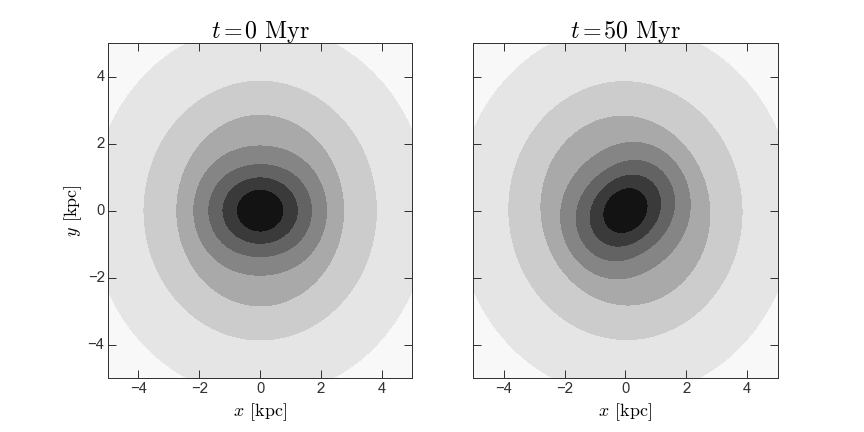
\includegraphics[width=\textwidth]{bar.png}
\label{fig:bar}
\end{center}
\end{figure*}
Try also making these same plots without the background potential. What is unphysical about this potential choice? 

\end{problem}

\begin{problem}

Write a function to generate initial conditions for star particles in a disk configuration. We will start by making a uniform, thin disk, meaning your initial conditions (in position-space) should look like those in Figure~\ref{fig:ics}. This is most easily done by sampling in radius and azimuthal angle (and for now, keeping z = 0), but be careful: sampling uniformly in radius will not give you a uniform disk density! Set the star velocities by assuming they are on circular orbits in the background potential (the Isochrone potential), for which you can analytically derive a circular velocity curve. You can test that you've set up you initial conditions properly by setting $\epsilon=0$ and integrating several of these orbits for a few dynamical times. They should all remain on circular orbits. 

\begin{figure*}[!h]
\begin{center}
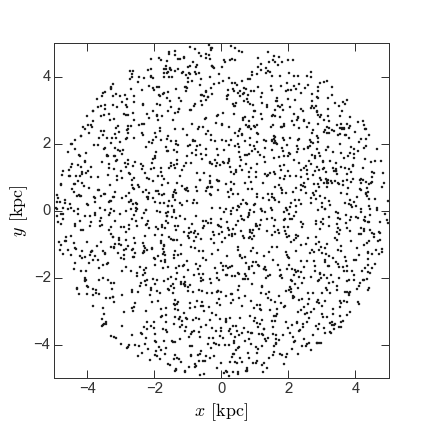
\includegraphics[width=0.5\textwidth]{ics.png}
\label{fig:ics}
\end{center}
\end{figure*}

\end{problem}

\begin{problem}

Before we integrate orbits, we will add one slight modification to the bar acceleration function. We will want to slowly ramp up the strength of the bar over a few orbital times so that the orbits adapt smoothly to the perturbing potential. Implement this by slowly increasing the bar strength $\epsilon$ from 0 to the specified parameter values over $\sim$1000 time steps.

Generate a set of 1000 initial conditions using your function from the previous problem over the range $r\in(0,8)$. Using a timestep set to $dt = 0.5$, integrate the orbits of these particles for 10000 steps in the total (Isochrone + bar) potential defined in Problem 1 with each of the parameter choices defined in Table 1. For each set of parameters, plot:
\begin{itemize}
\item the particle positions at the end of the integration time,
\item the density of particles in radial bins (a histogram of the radii).
\end{itemize}
Can you identify the Lindblad resonances? What are they? Co-rotation radius? How does the morphology of the disk change with $\epsilon$? How does the morphology of the disk change with $\Omega_p$?

For one of the parameter choices, we will now work the other direction to try to measure the pattern speed of the bar from stars trapped at the outer Lindblad resonance. What is the condition for a Lindblad resonance? For the last row parameter set, select stars around the outer Lindblad resonance. Measure the radial and azimuthal periods of these stars and compute the pattern speed from these periods. How do these measured pattern speeds compare to the ``true'' (input) value?

\begin{table}
\centering
\begin{tabular}{c c c}
$\epsilon$ & $\Omega_p$ & $a$ \\
\hline
0.01 & 0.02 & 2.5 \\
0.02 & 0.02 & 2.5 \\
0.08 & 0.02 & 2.5 \\
0.1 & 0.02 & 2.5 \\
0.01 & 0.1 & 2.5 \\
0.02 & 0.1 & 2.5 \\
0.08 & 0.1 & 2.5 \\
0.1 & 0.1 & 2.5 \\
0.01 & 0.2 & 2.5 \\
0.02 & 0.2 & 2.5 \\
0.08 & 0.2 & 2.5 \\
0.1 & 0.2 & 2.5 
\end{tabular}
\caption{Bar potential parameters.}
\end{table}

\end{problem}

\begin{problem}

For this final problem, your goal is to destroy a disk. We will assume the background potential is just the Isochrone potential from the first problem (not a very good assumption -- if you are up for it, use a disk-like potential instead, but this will require modifying your initial condition generator). Using your function from Problem 2, set up a new disk of 1000 particles with no scale height (e.g., again, keep $z=0$ for all particles) from $r\in(0,10)$. We're now going to drop perturbers into the disk with a variety of parameter choices. To start with, send a point mass flying through the center of the disk on an unbound orbit (but still a reasonable velocity) with ``mass'' $GM = 0.1$ (e.g., a 10-to-1 merger). What happens to the disk? 

Do this again, but instead of sending the mass through the center of the disk, set the impact parameter to 15. Using the impulse approximation (Section 8.2 in B\&T), estimate the energy input in to the disk particle orbits. Using your numerical results, compute the change in energy after the point mass has flown by. Do they agree?

Now, instead of sending the point mass through on an unbound orbit, we will set up the point mass on several different bound orbits around the disk. Try this for orbits with initial conditions:
\begin{table}
\centering
\begin{tabular}{c c c c c c c}
ID & $x$ & $y$ & $z$ & $v_x$ & $v_y$ & $v_z$ \\
\hline
c1 & 15 & 0 & 0 & 0 & 0.000 & 0.250 \\ % near-circular
c2 & 15 & 0 & 0 & 0 & 0.096 & 0.231 \\
c3 & 15 & 0 & 0 & 0 & 0.177 & 0.177 \\ 
c4 & 15 & 0 & 0 & 0 & 0.231 & 0.096 \\
c5 & 15 & 0 & 0 & 0 & 0.250 & 0.000 \\
e1 & 15 & 0 & 0 & 0 & 0.000 & 0.130 \\ % eccentric
e2 & 15 & 0 & 0 & 0 & 0.050 & 0.120 \\ 
e3 & 15 & 0 & 0 & 0 & 0.092 & 0.092 \\ 
e4 & 15 & 0 & 0 & 0 & 0.120 & 0.050 \\ 
e5 & 15 & 0 & 0 & 0 & 0.130 & 0.000
\end{tabular}
\caption{Satellite galaxy perturber initial conditions.}
\end{table}
Integrate for 10000 steps with a timestep dt=0.5. 

Make plots of the particle positions (in the $x-y$ plane) at the final timestep for all of the above. Label these plots by the initial conditions ID (see Table 2). How does the morphology of the disk depend on the inclination angle of the perturbing mass? Repeat the above for a perturber 10 times less massive. You do not need to re-make plots for this case, just comment on how much (qualitatively) this changes things. Given that real satellite galaxies are not point masses, how will this change things? What other dynamical processes are we missing in this extremely simplified demo that may be important?

\end{problem}

\end{document}

%\begin{figure*}[!h]
%\begin{center}
%\includegraphics[width=\textwidth]{PATH}
%\caption{ CAPTION }\label{fig:FIGNAME}
%\end{center}
%\end{figure*}